\documentclass[tikz,border=2pt]{standalone}
\usetikzlibrary{arrows.meta,positioning,fit,calc}

\begin{document}
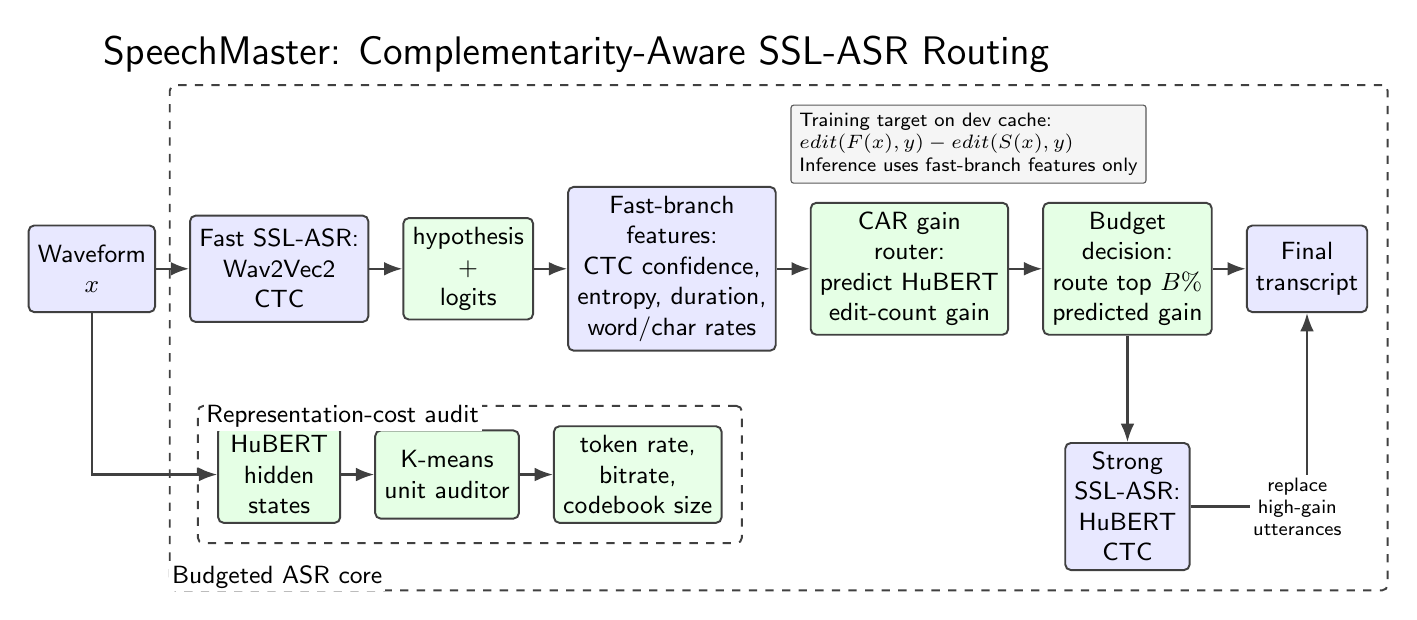
\begin{tikzpicture}[
    font=\small\sffamily,
    node distance=0.50cm and 0.42cm,
    block/.style={draw=black!75, line width=0.7pt, rounded corners=2pt,
        align=center, fill=blue!9, minimum height=1.10cm, minimum width=1.82cm},
    smallblock/.style={draw=black!75, line width=0.7pt, rounded corners=2pt,
        align=center, fill=green!9, minimum height=0.98cm, minimum width=1.30cm},
    wideblock/.style={draw=black!75, line width=0.7pt, rounded corners=2pt,
        align=center, fill=green!10, minimum height=1.12cm, minimum width=1.95cm},
    note/.style={draw=black!65, fill=gray!8, align=left, font=\scriptsize\sffamily,
        rounded corners=1pt, inner sep=3pt},
    group/.style={draw=black!75, dashed, line width=0.7pt, rounded corners=2pt, inner sep=7pt},
    arrow/.style={-Latex, line width=0.8pt, draw=black!75}
]

\node[font=\Large\sffamily] (title) at (6.15, 2.72)
    {SpeechMaster: Complementarity-Aware SSL-ASR Routing};

\node[block, minimum width=1.58cm] (audio) at (0, 0) {Waveform\\$x$};
\node[block, right=of audio, minimum width=1.88cm, minimum height=1.35cm] (fast)
    {Fast SSL-ASR:\\Wav2Vec2\\CTC};
\node[smallblock, right=of fast] (logits) {hypothesis\\+\\logits};
\node[block, right=of logits, minimum width=1.82cm, minimum height=1.35cm] (features)
    {Fast-branch\\features:\\CTC confidence,\\entropy, duration,\\word/char rates};
\node[wideblock, right=of features] (router)
    {CAR gain\\router:\\predict HuBERT\\edit-count gain};
\node[wideblock, right=of router] (budget)
    {Budget\\decision:\\route top $B\%$\\predicted gain};
\node[block, right=of budget, minimum width=1.35cm] (final)
    {Final\\transcript};

\node[note, above=0.23cm of router, xshift=0.75cm] (target)
    {Training target on dev cache:\\
     $edit(F(x),y)-edit(S(x),y)$\\
     Inference uses fast-branch features only};

\node[block, below=1.35cm of budget, minimum width=1.55cm, minimum height=1.22cm] (strong)
    {Strong\\SSL-ASR:\\HuBERT\\CTC};

\node[wideblock, below=1.30cm of fast, minimum width=1.55cm] (states)
    {HuBERT\\hidden\\states};
\node[wideblock, right=of states, minimum width=1.55cm] (kmeans)
    {K-means\\unit auditor};
\node[smallblock, right=of kmeans, minimum width=1.70cm] (rates)
    {token rate,\\bitrate,\\codebook size};

\draw[arrow] (audio) -- (fast);
\draw[arrow] (fast) -- (logits);
\draw[arrow] (logits) -- (features);
\draw[arrow] (features) -- (router);
\draw[arrow] (router) -- (budget);
\draw[arrow] (budget) -- (final);
\draw[arrow] (budget) -- (strong);
\draw[arrow] (strong.east) -| node[pos=0.24, right=1pt, align=center,
    font=\scriptsize\sffamily, fill=white, inner sep=1pt]
    {replace\\high-gain\\utterances} (final.south);

\draw[arrow] (audio.south) |- (states.west);
\draw[arrow] (states) -- (kmeans);
\draw[arrow] (kmeans) -- (rates);

\node[group, fit=(fast)(logits)(features)(router)(budget)(final)(target)(strong),
    label={[anchor=south west, font=\small\sffamily, fill=white, inner sep=1pt]south west:Budgeted ASR core}] {};
\node[group, fit=(states)(kmeans)(rates)] (unitgroup) {};
\node[font=\small\sffamily, fill=white, inner sep=1pt, anchor=west]
    at ($(unitgroup.north west)+(0.08,-0.15)$) {Representation-cost audit};

\end{tikzpicture}
\end{document}
